\documentclass{report}

% Custom language settings. In this case for Portuguese
\usepackage[portuguese]{babel}

% Package for support listings
\usepackage{listings}

% Package for support math
\usepackage{amsmath}

% Package for define some colors
\usepackage{xcolor}

% para incluir imagens e tratar de modo adequado endereços url
\usepackage{graphicx,url}

% para juntar multiplas linhas em tabelas
\usepackage{multirow}

% para poder rodar páginas
\usepackage{pdflscape}

% para incluir figuras do tipo eps
\usepackage{epsfig}

% Define some colors - Begin
\definecolor{ListingColorKeyWord}{rgb}{0, 0.5, 0}
\definecolor{ListingColorComment}{rgb}{0.0, 0.0, 0.6}
\definecolor{ListingColorIdentifier}{rgb}{0.5, 0.12, 0.10}
\definecolor{ListingColorEmphasize}{rgb}{0, 1, 1}

\definecolor{ListingColorBreakLine}{rgb}{0.5, 0.12, 0.10}

\definecolor{ListingColorDelimJSON}{rgb}{0, 0, 0}
\colorlet{ListingColorPunctJSON}{red!60!black}

\colorlet{HyperRefColorLink}{red!100}
\colorlet{HyperRefColorAnchor}{black!100} 
\colorlet{HyperRefColorCite}{green!100}
\colorlet{HyperRefColorFile}{cyan!100}
\colorlet{HyperRefColorMenu}{red!100}
\colorlet{HyperRefColorRun}{cyan!100}
\colorlet{HyperRefColorUrl}{magenta!100}

\definecolor{HyperRefColorBorderLink}{rgb}{1, 0, 0}
\definecolor{HyperRefColorBorderCite}{rgb}{0, 1, 0}
\definecolor{HyperRefColorBorderFile}{rgb}{0, 0.5, 0.5}
\definecolor{HyperRefColorBorderMenu}{rgb}{1, 0, 0}
\definecolor{HyperRefColorBorderRun}{rgb}{0.7, 0.7, 0.7}
\definecolor{HyperRefColorBorderUrl}{rgb}{0, 1, 1}

\colorlet{HyperRefColorWhite}{white!100}

% Define some colors - End

\usepackage[automake, acronym, toc, translate=false]{glossaries}

\usepackage{fancyvrb}

\usepackage{hyperref}
\hypersetup{
	colorlinks=true,
	linkcolor=HyperRefColorLink,
	anchorcolor=HyperRefColorAnchor, 
	citecolor=HyperRefColorCite,
	filecolor=HyperRefColorFile,
	menucolor=HyperRefColorMenu,
	runcolor=HyperRefColorRun,
	urlcolor=HyperRefColorLink,
	%allcolors=HyperRefColorWhite,
	citebordercolor=HyperRefColorBorderCite,
	filebordercolor=HyperRefColorBorderFile,
	linkbordercolor=HyperRefColorBorderLink,
	menubordercolor=HyperRefColorBorderMenu,
	urlbordercolor=HyperRefColorBorderUrl,
	runbordercolor=HyperRefColorBorderRun,
	%allbordercolors=HyperRefColorWhite,
}

% Change some of the default names used in indexes - Begin

% Adpated from the template used in the course "Projeto" from LEIM
\newcommand{\noNumChapterInIndex}[1]{
   \chapter*{#1}
   \addcontentsline{toc}{chapter}{#1}
}

\newcommand{\myPrefaceChapter}[1]{
   \noNumChapterInIndex{#1}
}

\renewcommand{\lstlistingname}{Listagem}

\renewcommand{\lstlistlistingname}{Índice de Listagens}

\renewcommand{\acronymname}{Lista de Acrónimos}

\addto\captionsportuges{
    \renewcommand{\chaptername}{Capítulo}
}

\setlength{\headheight}{15pt}

% Change some of the default names used in indexes - End

% Settings to be used when showing a listing for the Java language
\lstset{
	language=Java,
	keywordstyle={\color{ListingColorKeyWord}\bfseries},
	commentstyle=\color{ListingColorComment},
	identifierstyle=\color{ListingColorIdentifier},
	basicstyle=\ttfamily,
	frame=single,
	showstringspaces=false,
	numbers=left,
	tabsize=2,
	breaklines=true,
	postbreak=\mbox{\textcolor{ListingColorBreakLine}{$\hookrightarrow$}},
}

% Settings to be used when showing a listing for the Python language
\lstset{
	language=Python,
	keywordstyle={\color{ListingColorKeyWord}\bfseries},
	commentstyle=\color{ListingColorComment},
	identifierstyle=\color{ListingColorIdentifier},
	basicstyle=\ttfamily,
	frame=single,
	showstringspaces=false,
	numbers=left,
	tabsize=2,
	breaklines=true,
	postbreak=\mbox{\textcolor{ListingColorBreakLine}{$\hookrightarrow$}},
}

% Settings to be used when showing a listing for the Linux Bash shell script language
\lstset{
	language=Bash,
	keywordstyle={\color{ListingColorKeyWord}\bfseries},
	commentstyle=\color{ListingColorComment},
	identifierstyle=\color{ListingColorIdentifier},
	basicstyle=\ttfamily,
	frame=single,
	showstringspaces=false,
	numbers=left,
	tabsize=2,
	breaklines=true,
	emph={echo},
	postbreak=\mbox{\textcolor{ListingColorBreakLine}{$\hookrightarrow$}},
}

% Settings to be used when showing a listing for the XML language
\lstset{
	language=XML,
	emphstyle={\color{ListingColorEmphasize}\bfseries},
	commentstyle=\color{ListingColorComment},
	emph={Config, DataBase, host, port, db, username, password},
}

%Declare a new language. In this case JSON
\lstdefinelanguage{JSON}{
	basicstyle=\normalfont\ttfamily,
    numbers=left,
    numberstyle=\scriptsize,
    stepnumber=1,
    numbersep=8pt,
	frame=single,
	showstringspaces=false,
	numbers=left,
	tabsize=2,
	breaklines=true,
	xleftmargin=21pt,
	postbreak=\mbox{\textcolor{ListingColorBreakLine}{$\hookrightarrow$}},
	literate=
     *{:}{{{\color{ListingColorPunctJSON}{:}}}}{1}
      {,}{{{\color{ListingColorPunctJSON}{,}}}}{1}
      {\{}{{{\color{ListingColorDelimJSON}{\{}}}}{1}
      {\}}{{{\color{ListingColorDelimJSON}{\}}}}}{1}
      {[}{{{\color{ListingColorDelimJSON}{[}}}}{1}
      {]}{{{\color{ListingColorDelimJSON}{]}}}}{1},
}

\makeglossaries

\newacronym{asv}{ASV}{\textit{Autonomous Surface Vehicle}}
\newacronym{usv}{USV}{\textit{Unmanned Surface Vehicle}}
\newacronym{usb}{USB}{\textit{Universal Serial Bus}}


\begin{document}

% The listing number are indexed to the chapter name
\counterwithin{lstlisting}{chapter}

\tableofcontents

\cleardoublepage
\addcontentsline{toc}{chapter}{\listfigurename}
\listoffigures

\cleardoublepage
\addcontentsline{toc}{chapter}{\listtablename}
\listoftables

\cleardoublepage
\addcontentsline{toc}{chapter}{\lstlistlistingname}
\lstlistoflistings

\printglossaries

\chapter{Linguagem Python}
\label{ch:LangPython}

Na Listagem \ref{lst:PythonHardCoded} pode-se observar um exemplo (\textit{hard coded}) de uma listagem em Python.

\begin{lstlisting}[
	language=Python,
	caption=Exemplo em \texttt{Python},
	label=lst:PythonHardCoded]
# Declaring a float variable
myfloat = 7.0
print(myfloat) # Print the variable
myfloat = float(7)
print(myfloat)
\end{lstlisting}

Na Listagem \ref{lst:Python} pode-se observar um exemplo (localizado num ficheiro) de uma listagem em Python.

\lstinputlisting[
	language=Python,
	caption=Hello World em \texttt{Python},
	label=lst:Python,
	%firstline=5
]
{Hello.py}

\chapter{Linguagem Java}
\label{ch:LangJava}

A versão do exemplo \textbf{Hello World}, localizado num ficheiro e escrito na linguagem Java, é apresentada na Listagem \ref{lst:Java}.

\lstinputlisting[
	language=Java,
	caption=Hello World em \texttt{Java},
	label=lst:Java,
	%firstline=5
]
{Hello.java}

A Listagem \ref{lst:JavaVer2} apresenta um segundo exexmplo de uma listagem que apenas mostra parte de um ficheiro, nomeadamente a função \texttt{main(String[] args)}. É igualmente possível observar que quando uma linha de código sai das 
margens do texto é inserida de forma ``automática'' uma quebra de linha.

\lstinputlisting[
	language=Java,
	caption=Hello World em \texttt{Java} com recolha de nome,
	label=lst:JavaVer2,
	linerange={6-15}
]
{Hello-Ver2.java}

A listagem \ref{lst:JavaVer3} apresenta todo o programa mas exclui as linhas correspondentes aos \texttt{import}.

\lstinputlisting[
	language=Java,
	caption=Hello World em \texttt{Java} com recolha de nome - Programa completo,
	label=lst:JavaVer3,
	firstline=5
]
{Hello-Ver2.java}

\chapter{Linguagem Bash}
\label{ch:LangBash}

A Listagem \ref{lst:Bash} apresenta o conteúdo do ficheiro que suporta o exemplo \textbf{Hello World} escrito em Bash.

\lstinputlisting[
	language=Bash,
	caption=Hello World em \texttt{Bash},
	label=lst:Bash,
	%firstline=5
]
{Hello.sh}

\chapter{Linguagem XML}
\label{ch:LangXML}

Um exemplo de listagem, em \texttt{XML}, que está localizado num ficheiro e apresentado na Listagem \ref{lst:XML}.

\lstinputlisting[
	language=XML,
	caption=Exemplo em \texttt{XML},
	label=lst:XML,
	%firstline=5
]
{htconfig.xml}

\chapter{Linguagem JSON}
\label{ch:LangJSON}

Um exemplo de listagem, em \texttt{JSON}, que está localizado num ficheiro e apresentado na Listagem \ref{lst:JSON}.

\lstinputlisting[
	language=JSON,
	caption=Exemplo em \texttt{JSON},
	label=lst:JSON,
	%firstline=5
]
{htconfig.json}

\chapter{Gestão de Acrónimos}
\label{ch:ManAcronym}

O \LaTeX permite gerir acrónimos de forma automática. O primeio passo consiste em criar uma lista de acrónimos.
A lista de acrónimos é um ficheiro de texto com entradas do tipo:

\begin{verbatim}
	\newacronym{usb}{USB}{Universal Serial Bus}
\end{verbatim}


Para utilizar um acrónimo utiliza-se a expressão \Verb|\gls{nome}|. No primeira utilização o acrónimo é expandido 
e nas seguintes utilizações aparece apenas a sigla do acrónimo. Por exemplo, \gls{usb} e da segunda 
referência \gls{usb}.

No entanto, existem situações em pode ser necessário ter um controlo mais ``fino" para a expansão dos acrónimos. 
Para tal pode-se utilizar uma das seguintes expressões \LaTeX:

\begin{itemize}
	\item \Verb|\acrlong{nome}| -- para obter a definição do acrónimo
	\item \Verb|\acrshort{nome}| -- para obter a sigla do acrónimo
	\item \Verb|\acrfull{nome}| -- para obter a definição e sigla do acrónimo
\end{itemize}

No caso do acrónimo \textbf{usb} a utilização das expressões anteriores seria:

\begin{itemize}
	\item \acrlong{usb} -- para obter a definição do acrónimo
	\item \acrshort{usb} -- para obter a sigla do acrónimo
	\item \acrfull{usb} -- para obter a definição e sigla do acrónimo
\end{itemize}

Outros acrónimos que estão definidos são \gls{asv} e \gls{usv}. Que podem ser referidos várias vezes no texto: \gls{asv} e \gls{usv}.


\chapter{Figuras e Tabelas}
\label{ch:Misch}

O \LaTeX permite gerir a lista de figuras e tabelas de forma automática. O primeio passo consiste em criar as
 devidas imagems e tabelas, associando a cada uma delas um identificador único.

Por exemplo, a Tabela \ref{tab:umaTabela} apresenta os dados obtidos na experiência \ldots
\begin{table}[h]
	\centering
	\caption{Uma tabela}
	\begin{tabular}{ c c c c }
		\hline \hline
		$c_1$ & $c_2$ & $c_3$ & $\sum_{i=1} c_i$ \\
		\hline \hline
		$1$ & $2$ & $3$ & $6$ \\
		$1.1$ & $2.2$ & $3.3$ & $6.6$ \\
		\hline \hline
	\end{tabular}
	\label{tab:umaTabela}
\end{table}

A Tabela \ref{tab:umaTabela} é outro exemplo de uma tabela com barras verticais a separar as várias colunas.

\begin{table}[h]
	\centering
	\caption{Outra tabela com barras verticais}
	\begin{tabular}{ c|c|c|c }
		\hline \hline
		$c_1$ & $c_2$ & $c_3$ & $\sum_{i=1} c_i$ \\
		\hline \hline
		$1$ & $2$ & $3$ & $6$ \\
		$1.1$ & $2.2$ & $3.3$ & $6.6$ \\
		\hline \hline
	\end{tabular}
	\label{tab:outraTabela}
\end{table}

Para além de tabelas também é possivel apresentar figuras. Por exemplo, a Figura \ref{fig:umafigura} descreve \ldots
\begin{figure}[h]
	\centering
	
\includegraphics[width=2cm]{./fig_logo_ISEL}
	\caption[Uma figura com duas legendas]{Uma figura com duas legendas. A versão curta apenas aparece no índice de figuras}
	\label{fig:umafigura}
\end{figure}

\paragraph{Atenção.} Todas as tabelas e figuras, e.g., diagramas, imagens ilustrativas da aplicação em funcionamento, têm que ser devidamente enquadradas no texto antes de serem apresentadas e esse enquadramento inclui uma explicação da imagem apresentada e eventuais conclusões (interpretações) a tirar dessa imagem.

\mbox{} \\

A Figura \ref{fig:umafiguraR} apresenta um exemplo de uma figura que é apresentada numa página rodada 90º.

\begin{landscape}
\begin{figure}[h!]
	\centering
	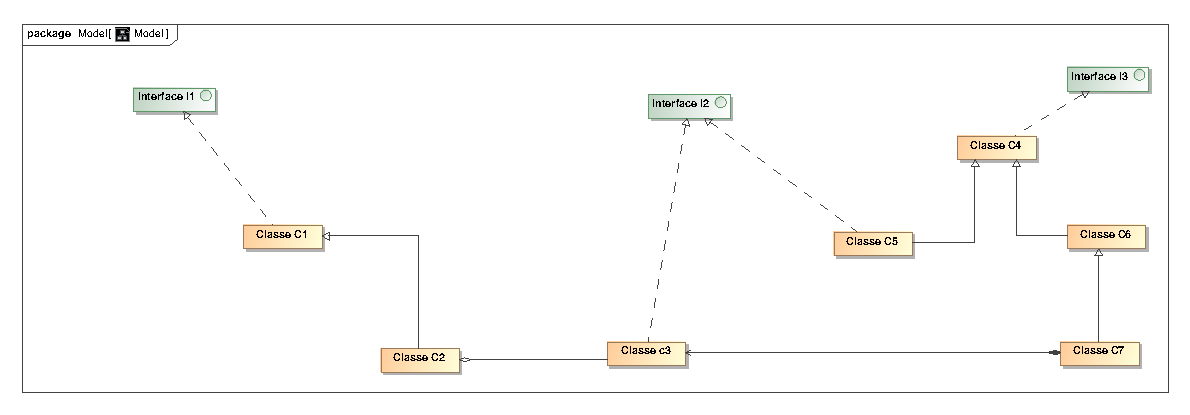
\includegraphics{./Model.eps}
	\caption{Figura rodada}
	\label{fig:umafiguraR}
\end{figure}
\end{landscape}

E mais texto depois da figura.


\end{document}